\q{30}{Neural Networks}

In this problem, you are given a simple network that uses the simple linear function $g(x) = mx + b$ (where $m$ and $b$ values are fixed) as the activation function (rather than, for example,  a sigmoid function). You will need to write the $L_2$ norm (squared) loss function, the partial derivative of the loss function, and the gradient descent update rule for certain weights.

\textbf{Single Neuron Example}

We have given you the answers for the loss function, partial derivative, and weight update rule for the following single neuron example. This example should help you understand how to structure your answers to the questions about the slightly more complex network on the following page.

\begin{figure}[h]
\centering
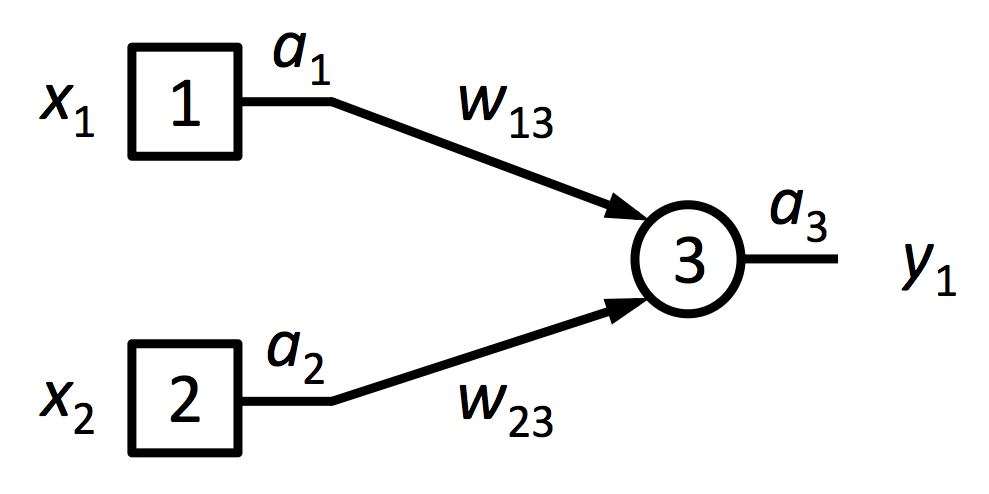
\includegraphics[width=0.25\linewidth]{figs/NN_1.png}
\end{figure}
\begin{flalign*}
a_1 &= x_1 &\\
a_2 &= x_2 &\\
a_3 &= m(w_{13}a_1+w_{23}a_2) + b &
\end{flalign*}
\textbf{Loss function}
\begin{flalign*}
Loss(\boldsymbol{w}) &= ||\boldsymbol{y}-\boldsymbol{h_w}(\boldsymbol{x})||_2^2 &\\
&= (y_1 - a_3)^2 &\\
&= (y_1 - m(w_{13}a_1+w_{23}a_2) - b)^2 &\\
&= (y_1 - m(w_{13}x_1+w_{23}x_2) - b)^2 &
\end{flalign*}
\textbf{Loss partial derivative}
\begin{flalign*}
\frac{\partial }{\partial w_{13}}Loss(\boldsymbol{w}) &= -2(y_1 - a_3) \frac{\partial a_3}{\partial w_{13}} &\\
&= -2(y_1 - a_3)ma_1 &\\
&= -2(y_1 - m(w_{13}x_1+w_{23}x_2) - b)mx_1 &
\end{flalign*}
\textbf{Weight update rule}
\begin{flalign*}
w_{13} &\leftarrow w_{13} - \alpha \frac{\partial }{\partial w_{13}} Loss(\boldsymbol{w})&\\
&= w_{13} + \alpha 2(y_1 - m(w_{13}x_1+w_{23}x_2) - b)mx_1 &
\end{flalign*}

(Question continued on next page)

\newpage
\textbf{Simple Neural Network with Linear Activation Function}

Given the following neural network (again, using the simple linear activation function $g(x) = mx + b$):

\begin{figure}[h]
\centering
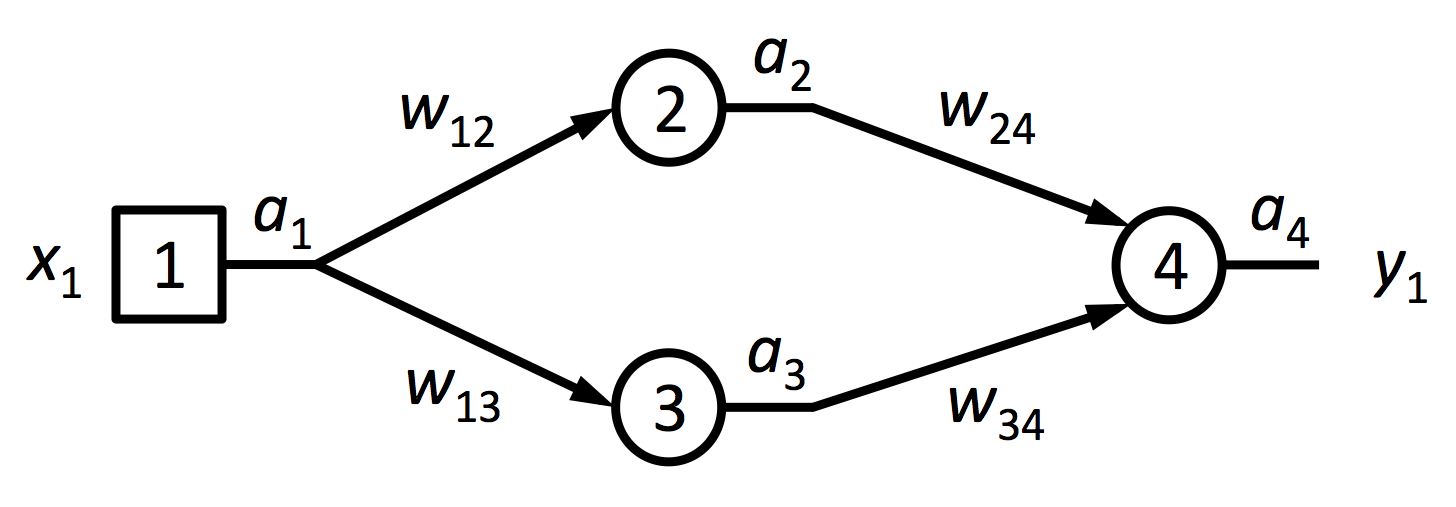
\includegraphics[width=0.4\linewidth]{figs/NN_2.png}
\end{figure}

\begin{question}{[5 pts]}
Write the loss function, $Loss(\boldsymbol{w})$, in terms of $x_1$, $y_1$, $w_{12}$, $w_{13}$, $w_{24}$, $w_{34}$, $m$, and $b$.

\begin{minipage}{\textwidth}
    \solution{} {\begin{align*}
    Loss(\boldsymbol{w}) &= (y_1-a_4)^2\\
    &= (y_1-m(w_{24}a_2+w_{34}a_3)-b)^2\\
    &= (y_1-m(w_{24}(mw_{12}a_1+b)+w_{34}(mw_{13}a_1+b))-b)^2\\
    &= (y_1-m^2w_{12}w_{24}x_1-mw_{24}b-m^2w_{13}w_{34}x_1-mw_{34}b-b)^2
    \end{align*}
    }
\end{minipage}

\end{question}

\begin{question}{[5 pts]}
Write the derivative of the loss function with respect to $w_{24}$, $\frac{\partial}{\partial w_{24}} Loss(\boldsymbol{w})$, in terms of $x_1$, $y_1$, $w_{12}$, $w_{13}$, $w_{24}$, $w_{34}$, $m$, and $b$.

\begin{minipage}{\textwidth}
    \solution{} {\begin{align*}
    \frac{\partial}{\partial w_{24}}Loss(\boldsymbol{w}) &= -2(y_1-a_4)\frac{\partial a_4}{\partial w_{24}}\\
    &= -2ma_2(y_1-a_4)\\
    &= -2m(mw_{12}x_1+b)(y_1-m^2w_{12}w_{24}x_1-mw_{24}b-m^2w_{13}w_{34}x_1-mw_{34}b-b)
    \end{align*}
    }
\end{minipage}

\end{question}

\begin{question}{[2 pts]}
Write the gradient descent update rule for $w_{24}$ with step size $\alpha$ in terms of $\alpha$ $x_1$, $y_1$, $w_{12}$, $w_{13}$, $w_{24}$, $w_{34}$, $m$, and $b$.

\begin{minipage}{\textwidth}
    \solution{} {\begin{align*}
    w_{24} &\leftarrow w_{24}-\alpha\frac{\partial}{\partial w_{24}} Loss(\boldsymbol{w})\\
    &= w_{24}+2\alpha m(mw_{12}x_1+b)(y_1-m^2w_{12}w_{24}x_1-mw_{24}b-m^2w_{13}w_{34}x_1-mw_{34}b-b)
    \end{align*}
    }
\end{minipage}

\end{question}

\begin{question}{[5 pts]}
Write the derivative of the loss function with respect to $w_{12}$, $\frac{\partial}{\partial w_{12}} Loss(\boldsymbol{w})$, in terms of $x_1$, $y_1$, $w_{12}$, $w_{13}$, $w_{24}$, $w_{34}$, $m$, and $b$.

\begin{minipage}{\textwidth}
    \solution{} {\begin{align*}
    \frac{\partial}{\partial w_{12}}Loss(\boldsymbol{w}) &= -2(y_1-a_4)\frac{\partial a_4}{\partial w_{12}}\\
    &= -2(y_1-a_4)(mw_{24}\frac{\partial a_2}{\partial w_{12}}+mw_{34}\frac{\partial a_3}{\partial w_{12}})\\
    &= -2(y_1-a_4)(mx_1+0)\\
    &= -2mx_1(y_1-m^2w_{12}w_{24}x_1-mw_{24}b-m^2w_{13}w_{34}x_1-mw_{34}b-b)
    \end{align*}
    }
\end{minipage}

\end{question}

\begin{question}{[2 pts]}
Write the gradient descent update rule for $w_{12}$ with step size $\alpha$ in terms of $\alpha$ $x_1$, $y_1$, $w_{12}$, $w_{13}$, $w_{24}$, $w_{34}$, $m$, and $b$.

\begin{minipage}{\textwidth}
    \solution{} {\begin{align*}
    w_{12} &\leftarrow w_{12}-\alpha\frac{\partial}{\partial w_{12}} Loss(\boldsymbol{w})\\
    &= w_{12}+2\alpha mx_1(y_1-m^2w_{12}w_{24}x_1-mw_{24}b-m^2w_{13}w_{34}x_1-mw_{34}b-b)
    \end{align*}
    }
\end{minipage}
\end{question}

\newpage

\begin{question}{[3 pts]}
Because this network has a linear activation function, there is an equivalent network that has no hidden layers. 1) Draw a new (very simple) network that has no hidden layers but computes exactly the same function. 2) Write the new weight explicitly in terms of the $w_{12}$, $w_{13}$, $w_{24}$, $w_{34}$, $m$, and $b$. 3) You will need to adjust the linear activation function, $g_2(x) = m_2x + b_2$. Write the new $m_2$ and $b_2$ values in terms of $w_{12}$, $w_{13}$, $w_{24}$, $w_{34}$, $m$, and $b$.

\begin{minipage}{\textwidth}
    \solution{} {\begin{verbatim}
    x1 (1) a1 -----------> (2) a2', y1
                   w'
    \end{verbatim}
    \begin{align*}
    a2' &= a4\\
    &= m^2w_{12}w_{24}x_1+mw_{24}b+m^2w_{13}w_{34}x_1+mw_{34}b+b\\
    &= m^2(w_{12}w_{24}+w_{13}w_{34})x_1 + (mw_{24}b+mw_{34}b+b)\\
    w' &= w_{12}w_{24}+w_{13}w_{34}\\
    m_2 &= m^2\\
    b_2 &= mw_{24}b+mw_{34}b+b
    \end{align*}
    }
\end{minipage}
\end{question}

\textbf{General Neural Network with Linear Activation Function}

\vspace{3mm}
Consider a new neural network with $n$ input nodes, $n$ output nodes, one hidden layer with $h$ nodes, and the linear activation function $g(x) = mx + b$ at each hidden and output node. The nodes between each layer are fully connected with weights $w_{ij}$ from the $i$-th input node to the $j$-th hidden node and weights $w_{jk}$ from the $j$-th hidden node to the $k$-th output node.

\vspace{3mm}
\begin{question}{[5 pts]}
Because this general network has a linear activation function, there is an equivalent network that has no hidden layers that computes exactly the same function. 1) Write an equation for the weight $w_{ik}$ from the $i$-th input node to the $k$-th output node explicitly in terms of the previous network weights ($w_{ij}$, $w_{jk}$), $m$, and $b$. 2) You will need to adjust the linear activation function, $g_2(x) = m_2x + b_2$. Write the new $m_2$ and $b_2$ values in terms of the previous network weights ($w_{ij}$, $w_{jk}$), $m$, and $b$.

\begin{minipage}{\textwidth}
    \solution{} {\begin{align*}
    y_k &= m\sum_{j=1}^h(w_{jk}(m\sum_{i=1}^n(w_{ij}x_i)+b))+b\\
    &= m^2\left(\sum_{j=1}^h\sum_{i=1}^n w_{ij}w_{jk}x_i\right) + \left(\sum_{j=1}^h\sum_{i=1}^n mw_{jk}b\right) + b\\
    w_{ik} &= \sum_{j=1}^h w_{ij}w_{jk}\\
    m_2 &= m^2\\
    b_{2,k} &= b\left(1+mn\sum_{j=1}^h w_{jk}\right)
    \end{align*}
    }
\end{minipage}
\end{question}

\begin{question}{[3 pts]}
What effect does removing the hidden layer from this general network have on the number of weights? Specifically, in terms of $n$ and $h$, how many weights are there before and after removing the hidden layer? Discuss in particular the case when $h << n$.

\begin{minipage}{\textwidth}
    \solution{} {
    \paragraph{} Before removing the hidden layer there are $hn$ weights on each side of it for a total of $2hn$ weights. After removing it, there are $n^2$ weights, one for each pair of input/output. When $h<<n$ this essentially increases the number of weights by a factor of $\frac n2$.
    }
\end{minipage}

\end{question}




